\section{Extending the State Channel}

We explain the operation of a two-party state channel and then extend the functionality to multiple parties. A data structure that models the cash distribution after each hand is introduced. Lastly, a leave protocol is described that protects participants from accepting uncovered bets. 


\subsection{State Channels}
State channels are a way to think about blockchain interactions which could occur on-chain, but instead get conducted off the chain, without  increasing the risk of any participant. The most well known example of this strategy is the idea of payment channels in Bitcoin, which allow for instant fee-less payments to be sent directly between two parties \cite{coleman15}. 

The life-cycle of a state channel can be broken down into steps as depicted in figure \ref{pc_settle}:

\begin{figure}[!ht]
\centering
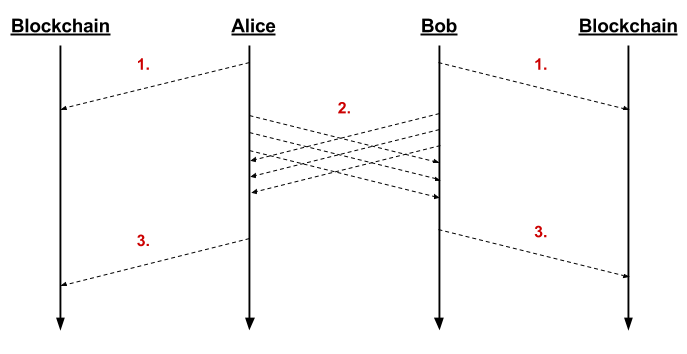
\includegraphics[width=3.0in]{images/settle.png}
\caption{A state channel netted by settlement.}
\label{pc_settle}
\end{figure}

\begin{enumerate}
\item Alice and Bob lock up some tokens by sending a transaction to the payment channel contract.
\item They can internally transfer value by signing receipts about new commitments and exchanging them. The receipts have to carry increasing sequence numbers and signatures.
\item Alice and Bob can release the bonded tokens by mutually agreeing (signing) on a resolution.
\end{enumerate}

Several reasons might hinder Alice and Bob from agreeing on a resolution, like malicious intentions or network connectivity. In this case the channel is closed through dispute, as depicted in figure \ref{pc_dispute}.

\begin{figure}[!ht]
\centering
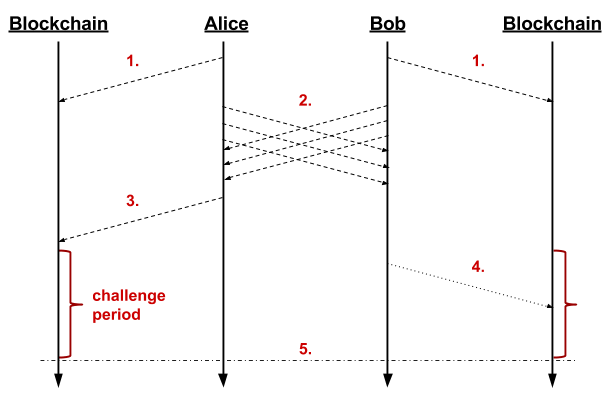
\includegraphics[width=3.0in]{images/dispute.png}
\caption{A state channel netted after dispute.}
\label{pc_dispute}
\end{figure}

\begin{enumerate}
\item Alice and Bob lock up some tokens by sending a transaction to the payment channel contract.
\item They can internally transfer value by signing receipts about new commitments and exchanging them. The receipts have to carry increasing sequence numbers and signatures.
\item If Alice or Bob stop cooperating, the latest receipt can always be submitted to the blockchain. This will trigger a challenge period.
\item During the challenge period each participant is incentivised to submit the receipt for the highest commitment of his opponent.
\item After the challenge period expires, the bonded tokens are released to Alice and Bob by the ratio of the receipts with highest sequence numbers.
\end{enumerate}

In effect, a state channel buffers the operations that would otherwise be written to the blockchain. Using a state channel decouples an application from the liveliness constraints of the blockchain without relaxing the security assumptions.

\subsection{multiparty State Channels}

An interaction of multiple participants could be modeled as a set of bilateral state channels from each player to each player. Yet, as the distribution of cash is not known beforehand, each channel would need to be funded with the full amount, resulting in a requirement of security deposits of \(O(n^2)\) tokens.

To be able to operate the channel with multiple parties and \(O(n)\) size of deposits, we define a commitment data structure as shown in figure \ref{mpc_round}. 

\begin{figure}[!ht]
\centering
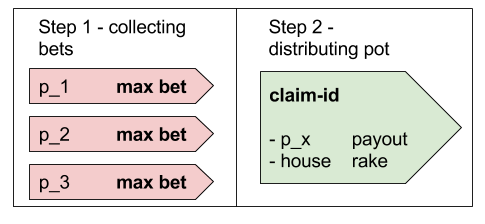
\includegraphics[width=2.5in]{images/bet.png}
\caption{Commitments and distribution}
\label{mpc_round}
\end{figure}

Commitments by participants carry a value, but do not have a specific recipient. Each higher value commitment by a participant replaces a lower one. When results of secure computation become available an oracle evaluates the data and issue a corresponding distribution receipt, reassigning the values from the participants' commitments to the winner(s) deducted from the multiparty computation.

Multiple rounds of commitments and distributions (hands played) can happen among the participants of the multiparty state channel. These rounds are numbered by a strictly increasing identifier (handId). Figure \ref{mpc_settle} depicts that, as long as all parties agree on a final settlement, the protocol is equivalent to the two-party channel:

\begin{figure}[!ht]
\centering
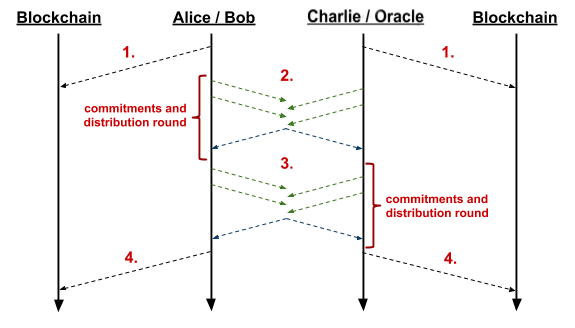
\includegraphics[width=3.0in]{images/multiSettle.png}
\caption{A multiparty state channel netted through settlement.}
\label{mpc_settle}
\end{figure}

\begin{enumerate}
\item Alice, Bob and Charlie lock up some tokens by sending a transaction to the multiparty state channel contract.
\item A round of commitment and distribution executes. In the round, the participants repeatedly bet value by signing receipts about new commitments and broadcasting them. The round is  closed by the distribution receipt, which awards the committed value to the winner(s).
\item participants can have multiple further rounds of commitment and distribution, as long as at least 2 participants stay solvent.
\item Alice, Bob and Charlie mutually agree on a resolution. The resolution sums up the value transferred over all rounds performed since the start of the channel. The smart contract evaluates the resolution and updates the balances of all participants. 
\end{enumerate}

Whenever the balances are update also the latest handId is updated in the state of the contract. This process is called netting. The netting can happen when all parties agree through resolution, or when there is disagreement, through dispute. The dispute is executed as depicted in figure \ref{mpc_dispute}.

\begin{figure}[!ht]
\centering
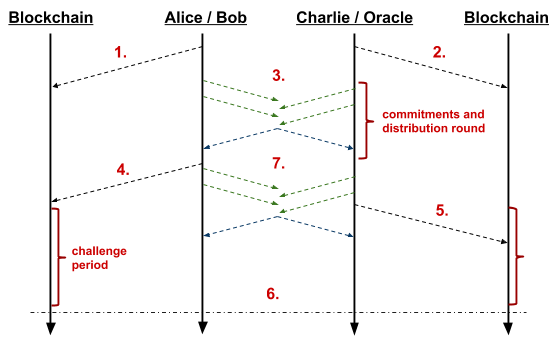
\includegraphics[width=3.0in]{images/multiDispute.png}
\caption{A multiparty state channel netted after dispute.}
\label{mpc_dispute}
\end{figure}

\begin{enumerate}
\item Alice, Bob lock up some tokens by sending a transaction to the multiparty state channel contract.
\item Charlie can join the channel later by also sending a transaction to the contract and also locking up some tokens.
\item A round of commitment and distribution executes. In the round, the participants repeatedly bet value by signing receipts about new commitments and broadcasting them. The round is  closed by the distribution receipt, which awards the committed value to the winner(s).
\item Bob signals to leave the state channel, but is unable to sign the resolution due to network issues. The challenge period is triggered in the contract.
\item The participants submit receipts of commitments and distributions to the contract.
\item The smart contract sums up the receipts over all rounds since the last netting and updates the balances of all participants. Once the netting progresses beyond the handId at which Bob signaled leaving, he is payed out and removed from the contract.
\item During the challenge period remaining solvent players can continue to execute rounds of commitments and distributions.
\end{enumerate}

\subsection{Asynchronous participation}

Rotation into a state channel requires no special protocol, once the deposit is placed, the participant can be interacted with.

Rotation out of a channel has the potential risk that a remaining party could be handed uncovered commitments by the leaving party after it has withdrawn its deposit already. To guard against this situation, we extend the on-chain state with the variables:


\begin{description}
\item[lastNettedHand (LNR):] describes the id of the last hand at which the channel has been netted. this is also the hand at which the balance of the participant is valid.
\item[exitHand:] each participant maintains this flag, which is initialized with 0 and stays unchanged until the participant signals to leave. At that point the participant requests a leave receipt from the oracle, which identifies the latest hand id in the channel. This receipt is submitted to the chain and sets the exit Hand of the participant.
\item[NettingRequestHand (NRH):] This variable tracks the id of the latest hand that has completed in the state channel. Yet, this variable is only updated in the contract if a participant of the state channel requests to leave.
\item[NettingRequestTime (NRT):] This variable is set to the current time simultaneously to NRH. It will be used to to measure the challenge period if a dispute arises.
\end{description}

Table \ref{fsm-table} shows the state transition of the channel from having an empty seat, to a player joining and playing, to netting and leave. 


\begin{table}[ht]
\centering
\caption{State transition of seat and table.}
\label{fsm-table}
\begin{tabular}{lccccc}
\hline
                 & \multicolumn{2}{c}{seat x} & \multicolumn{1}{l}{} & \multicolumn{1}{l}{} & \multicolumn{1}{l}{} \\ 
                 & balance     & exitHand     & LNH                  & NRH                  & NRT                  \\ \hline
1) empty         & 0           & 0            & y                    & y                    & 0                    \\
2) join          & 100         & 0            & y                    & y                    & 0                    \\
3) play          & 100         & 0            & y                    & y                    & 0                    \\
4) request leave & 100         & z            & y                    & z                    & 999                  \\
5) netting       & 80          & z            & z                    & z                    & 999                  \\
6) leave         & 0           & 0            & z                    & z                    & 0                    \\ \hline
\end{tabular}
\end{table}

Once the exitHand flag of a leaving participant is set in the contract, other participants can clearly judge to accept or reject receipts in the current round. When, either through agreement, or dispute, the channel is netted beyond a participants exitHand ( LNH >= exitHand ), the participant is payed out and removed from the channel. 
